\documentclass[tikz,border=9pt]{standalone}
\usepackage{amsmath,amssymb}
\usetikzlibrary{arrows.meta,positioning,calc}
\begin{document}
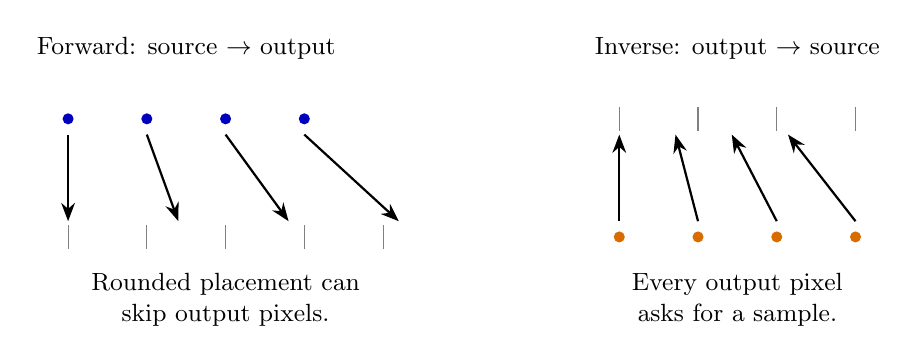
\begin{tikzpicture}[font=\small,arr/.style={-{Stealth},thick},box/.style={draw=blue!55!black,rounded corners,fill=blue!4,align=center,text width=2.9cm,minimum height=1.05cm}]

\node at (1.5,2.4){Forward: source $\to$ output};
\foreach \x in {0,1,2,3}{\fill[blue!75!black] (\x,1.5) circle(2pt);\draw[arr] (\x,1.3)--({1.4*\x},.2);}
\foreach \x in {0,1,2,3,4}{\draw[gray] (\x,-.15)--(\x,.15);}
\node[align=center] at (2,-.8){Rounded placement can\\skip output pixels.};
\begin{scope}[shift={(7,0)}]
\node at (1.5,2.4){Inverse: output $\to$ source};
\foreach \x in {0,1,2,3}{\fill[orange!85!black] (\x,0) circle(2pt);\draw[arr] (\x,.2)--({\x/1.4},1.3);}
\foreach \x in {0,1,2,3}{\draw[gray] (\x,1.35)--(\x,1.65);}
\node[align=center] at (1.5,-.8){Every output pixel\\asks for a sample.};
\end{scope}

\end{tikzpicture}
\end{document}
